% ======================================================================
% QIJ — WSOM+2026 submission
% Notation: psi = influence function; RF = receptive field (n_j counts,
% p_j = n_j/N); W = prototypes; V_tot = V_btw + V_win (identity, eq. 4).
% Figures: f3.pdf f2.pdf f7.pdf f9.pdf alongside this file.
% ======================================================================
\documentclass[runningheads]{llncs}

\usepackage[T1]{fontenc}
\usepackage{graphicx}
\usepackage{amsmath,amssymb}
\usepackage{mathtools}
\usepackage{url}
\usepackage{booktabs}

% --- notation ---
\newcommand{\ifl}{\psi}
\newcommand{\Vcell}{V_{\mathrm{btw}}}
\newcommand{\Vwithin}{V_{\mathrm{win}}}
\newcommand{\Vtotal}{V_{\mathrm{tot}}}
\newcommand{\Fhat}{\hat F}

\begin{document}

\title{Vector Quantization for Uncertainty Quantification: The Quantized Infinitesimal Jackknife}

\titlerunning{Vector Quantization for Uncertainty Quantification}
% ORCID iDs can be added via \orcidID{...} after each name if desired
\author{Josh Taylor\inst{1}\thanks{Corresponding author.} \and
Stella S. R. Offner\inst{1}}
\authorrunning{J. Taylor and S. S. R. Offner}
\institute{The University of Texas at Austin, Department of Astronomy and Oden Institute for Computational Engineering and Sciences, Austin, Texas, USA
\email{joshtaylor@utexas.edu}}

\maketitle

\begin{abstract}
Nonparametric confidence intervals (CIs) for a parameter estimate $T$ are commonly obtained by the bootstrap: recompute the estimate on $B$ resampled datasets and infer estimate uncertainty from the replicates. The bootstrap is the gold standard, but it costs $B$ evaluations of the estimator, prohibitive when a single fit is expensive, e.g.\ when $T$ must be found by numerical optimization rather than in closed form. 

We show that a fitted vector quantizer (VQ) offers a much cheaper route to similar intervals. The Quantized Infinitesimal Jackknife (QIJ) uses a
quantizer's $M$ receptive fields as perturbation scaffolding for the
uncertainty calculation, measuring how $\hat{T}$ responds when each field's
share of the data is perturbed (propagating these multinomial fluctuations through the measured responses), yielding the variance and skewness of the estimator's sampling distribution. This is like the infinitesimal jackknife (IJ), except the perturbation occurs across $M$ Voronoi regions, instead of $N$ sample observations. It recovers IJ as $M \to N$. No resampling occurs anywhere, and the number of estimator evaluations scales with $M$ rather than $B$. The underlying variance analysis applies to any VQ resolution. On two synthetic distributions (Pareto; multivariate $t$ in ten dimensions)
and an astronomical dataset (the galaxy Fundamental Plane), QIJ matches the
bootstrap's coverage and interval widths across eight estimands at a small
fraction of its computation.

%We show that a fitted vector quantizer offers a much cheaper route to the same intervals. The Quantized Infinitesimal Jackknife (QIJ) uses the quantizer's $M$ receptive fields (with counts $n_j$) as the variables of the uncertainty calculation: the estimator is re-expressed as a function of the counts, and QIJ measures how $T$ responds when each $n_j$ is perturbed, which is the natural impact of resampling on a VQ. This requires only $\mathcal{O}(M)$ evaluations of $T(X)$ in total, vs.\ $B \gg M{+}1$ in the standard bootstrap. We infer the variance and skewness of the estimate by propagating the counts' exactly known (multinomial) sampling fluctuations through the measured responses; both feed our VQ-enabled CIs, and no resampling occurs anywhere. On two synthetic distributions (Pareto; multivariate $t$ in ten dimensions) and an astronomical dataset (the galaxy Fundamental Plane), QIJ matches the bootstrap's coverage and interval widths at a small fraction of its computation.
\keywords{vector quantization \and uncertainty quantification \and confidence intervals \and influence functions \and bootstrap}
\end{abstract}


% ======================================================================
\section{Introduction}\label{sec:intro}
% ======================================================================

Vector quantization (VQ) compresses a dataset $X = \{x_i \in \mathbb{R}^d\}_{i=1}^N$ into $M \ll N$ prototypes $W = \{w_j\}_{j=1}^M$ to facilitate signal encoding, clustering, density representation \cite{graf2000}, and, through self-organizing maps and their descendants, topology-preserving visualizations. In this work, we assign VQ the task of constructing confidence intervals for an arbitrary parameter estimate  computed from $X$.

The bootstrap \cite{efron1979} is the gold standard for nonparametric interval estimation: recompute the estimator $T$ on $B$ resampled datasets, with $B$ in the hundreds to thousands, and infer CIs from the replicated sampling distribution of $T$. When a single evaluation of $T$ is expensive, e.g., the result of an optimizer-based fit, a profile likelihood, or an ensemble fit, those $B$ evaluations dominate the analysis. Since a VQ represents a large dataset compactly, one might expect its prototypes to stand in for the $N$ sample points during resampling; this works well for point estimates, but not for interval estimation. That is, in terms of uncertainty quantification, the quantizer prototypes are not just a smaller dataset from which to resample. Quantization suppresses precisely the sampling noise that interval estimation requires. We can, however, recover a notion of sampling variability by studying how resampling variance interacts with a VQ partition: there is variation in \emph{how many} points land in each region, and also in \emph{which} points represent each region. The VQ objective minimizes the second part by construction (if the VQ is trained properly); in this work we exploit multinomial models of the first to obtain CIs.

To achieve this, we replace explicit resampling with perturbation. Under bootstrap resampling, the counts $(n_1,\dots,n_M)$ of data in each region fluctuate acording to a multinomial covariance. Importantly, no simulation is required to learn it. The only unknown is how sensitive the estimator is to each changing count, and that is a derivative: perturb one region's share of the data, re-evaluate $T$, and record the response. Our Quantized Infinitesimal Jackknife (QIJ) does exactly this, via $\mathcal{O}(M)$ deterministic evaluations of $T$ in total, and propagates the counts' known covariance through these responses (the delta method), yielding the variance and skewness of $T$'s sampling distribution. The result is a VQ-based confidence interval with no resampling at any stage (Sect.~\ref{sec:method}).

These VQ-based confidence intervals are based on the observation that we can decompose an estimator $T$'s total variance into two parts. The first captures the estimator variance that would occur from distributing a resampling of points into the existing partition (i.e., Voronoi regions would obtain new counts), while the second describes estimator impact from within-region point variation. QIJ measures the first directly, and recovers the second from the same partition statistics. Crucially, decomposing at a different $M$ returns the same total (i.e., the total variance does not depend on the partition). We use this as a correctness check in Sect.~\ref{sec:results}.

\paragraph{Related work.} The infinitesimal jackknife originates with Jaeckel \cite{jaeckel1972}; Efron \cite{efron1982} connects it to the bootstrap. Wager et al.\ \cite{wager2014}, similarly motivated by an estimator too expensive to resample, apply it to random forests, though their derivative is taken with respect to individual observation weights, whereas ours is taken with respect to Voronoi masses. The Bag of Little Bootstraps \cite{kleiner2014} and $m$-out-of-$n$ subsampling \cite{bickel1997} reduce the size of each resample but still resample, and their approximation error is asymptotic and unobserved; QIJ never resamples, and its approximation error is a reported quantity. The influence-function machinery we rely on is classical robust statistics \cite{hampel1974,stefanski2002}.


% ======================================================================
\section{The Quantized Infinitesimal Jackknife}\label{sec:method}
% ======================================================================

\subsection{Setup: Voronoi Influence Functions}\label{sec:setup}

This section develops the perturbation calculus previewed above. 

Let $X=\{x_i\}_{i=1}^{N}$ be iid from $F$, let $\hat{F}$ be its empirical
distribution, and let $T$ be a functional on distributions, so that the
estimand is $\theta = T(F)$ and the estimator is its plug-in
$\hat{T} = T(\hat{F})$. The influence function of $T$ at $\hat{F}$ is
%
\begin{equation}\label{eq:if}
  \psi(x) \;=\; \lim_{\varepsilon \to 0}
  \frac{T\!\big((1-\varepsilon)\hat{F} + \varepsilon\,\delta_x\big) - T(\hat{F})}
       {\varepsilon},
\end{equation}
%
the derivative of $T$ in the direction of a point mass at $x$, i.e.\ how much
the estimate moves per unit of probability placed at $x$; it satisfies
$\sum_i \psi(x_i) = 0$. The classical linearization
$\hat{T} - \theta \approx \tfrac{1}{N}\sum_i \psi(x_i)$~\cite{vonmises1947,hampel1974}
underlies both the jackknife and the bootstrap, and gives
$\operatorname{Var}(\hat{T}) \approx \mathbb{E}[\psi^2]/N$.

We fit a vector quantizer with $M$ prototypes $W$ to the data. Each
prototype's Voronoi region is its receptive field (RF); RF~$j$ contains $n_j$
points, with mass fraction $p_j = n_j/N$ and $p = (p_1,\dots,p_M)$. The RF
influence $U_j$ is the derivative of $T$ at RF~$j$ with the point mass replaced by an equal spread of mass over the points of RF~$j$:
%
\begin{equation}\label{eq:Uj}
  U_j \;=\; \lim_{\varepsilon \to 0}
  \frac{T\!\Big((1-\varepsilon)\hat{F}
        + \frac{\varepsilon}{n_j}\sum_{i \in \mathrm{RF}_j} \delta_{x_i}\Big)
        - T(\hat{F})}{\varepsilon}
  \;=\; \frac{1}{n_j} \sum_{i \in \mathrm{RF}_j} \psi(x_i).
\end{equation}
%
The perturbation raises RF~$j$'s mass by $\varepsilon$ at the expense of the
others, reweighting every point inside RF~$j$ identically (never individually).
Since the derivative is linear in the direction perturbed, the response is the
average of the individual responses $\psi(x_i)$, which is the second equality.

Eq.~\eqref{eq:Uj} is the infinitesimal jackknife (IJ) of~\cite{jaeckel1972} with its perturbation space restricted to the $M$ receptive-field masses (instead of $N$ observation weights); $U_j$ is the IJ derivative applied to the RF-conditional mean influence. At $M = N$ each RF holds a
single point, $U_j = \psi(x_j)$, and \eqref{eq:identity} reduces to the classical infinitesimal jackknife variance $N^{-2}\sum_i \psi(x_i)^2$. At $M = 1$ the single RF gives $U_1 = 0$ and the entire variance sits in
$V_\mathrm{win}$. QIJ interpolates between these according to the
resolution of the quantizer.

% Let $X = \{x_i\}_{i=1}^N \stackrel{\mathrm{iid}}{\sim} F$ and let $\hat{F}$ denote the empirical distribution of $X$. We define the estimand as a functional $T$ on distributions, $\theta = T(F)$, and the estimator to be its plug-in $\hat{T} \coloneq T(F\hat{F})$. $T$'s influence function, denoted $\ifl$ throughout, is
% \begin{equation}\label{eq:influence}
% \ifl(x) \;=\; \lim_{\varepsilon \to 0}\frac{T\bigl((1-\varepsilon)G + \varepsilon\,\delta_x\bigr) - T(G)}{\varepsilon},
% \end{equation}
% which is the derivative of $T$ in the direction of a point mass at $x$ (i.e., it describes how much the estimate moves per unit of probability placed at $x$). Eq. \ref{eq:influence} evaluated at $G = F$ gives the population influence function. In what follows, we use its empirical counterpart $\psi(x) \coloneq \psi(x; \hat{F})$, which satisfies $\sum_i \psi(x_i) = 0$, since $\int \psi(·; G) dG = 0$ for any distribution $G$. The classical linearization $T(X) - \theta \approx \tfrac1N\sum_i \ifl(x_i)$ \cite{vonmises1947,hampel1974} underlies both the jackknife and the bootstrap, and gives $\mathrm{Var}\bigl(T(X)\bigr) \approx \tfrac1N\,\mathbb{E}[\ifl^2]$.

% To begin, we fit a vector quantizer with $M$ prototypes $W = \{w_j\}$ to the data. Each prototype's Voronoi region is its \emph{receptive field} (RF); RF $j$ contains $n_j$ data points, with mass fraction $p_j = n_j/N$ and $p = (p_1,\dots,p_M)$. Let $\hat{G}_j = (1/n_j) \sum_{i \in RF_j} \delta_{x_i}$ be the empirical measure of RF $j$ (a probability measure supported on RF $j$), so that $\hat{F} = \sum_j p_j\hat{G}_j$. 
% The observed masses form a point $p \in \Delta^{M-1}$ (the $M-1$ dimensional unit simplex). To perturb them we hold the regions and their contents fixed and vary the mixture weights: for $q \in \Delta^{M-1}$, set $\hat{F}_q = \sum_j q_j \hat{G}_j$ and $\tilde{T}(q) := T(\hat{F}_q)$. This is defined for every functional $T$, and returns the estimator at the observed masses, $\tilde{T}(p) = T(\hat{F}) = \hat{T}$. We define the \emph{RF influence} $U_j$ as the derivative of $T$ toward RF $j$:
% \begin{equation}\label{eq:Uj}
% %U_j \;=\; \frac{d}{d\varepsilon}\,T\bigl((1-\varepsilon)\,p + \varepsilon\, e_j\bigr)\Big|_{\varepsilon = 0}
% %\;=\; \frac{1}{n_j}\sum_{i \in \mathrm{RF}_j} \ifl(x_i),
% %U_j = \frac{d}{d\varepsilon}\, \tilde{T}((1−\varepsilon)p + \varepsilon e_j) \quad | \quad {\varepsilon=0} = (1/n_j) \sum_{i \in RF_j} \psi(x_i)
% U_j = \lim_{\varepsilon \to 0}
%   \frac{\tilde{T}\big((1-\varepsilon)\,p + \varepsilon\, e_j\big) - \tilde{T}(p)}{\varepsilon}
%   = \frac{1}{n_j} \sum_{i \in \mathrm{RF}_j} \psi(x_i)
% \end{equation}
% where $e_j \in \mathbb{R}^M$ is the $j$-th standard basis vector of the \emph{weight space}, i.e., the mass vector that places all weight on RF $j$ (note $e_j$ is unrelated to the data space $\mathbb{R}^d$). 

% The mixture in mass space maps to a mixture in distribution space: $\hat{F}_{(1-\varepsilon)p + \varepsilon e_j} = (1-\varepsilon)\hat{F} + \varepsilon \hat{G}_j$, where $\hat{G}_j = (1/n_j) \sum_{i \in RF_j} \delta_{x_i}$ is the empirical measure of RF $j$. Differentiating at $\varepsilon = 0$ and using $\int \psi dF\hat{F} = 0$ gives the second equality. Intuitively, the perturbation raises RF $j$'s mass at the expense of the others while reweighting every point inside RF $j$ identically, never individually; the response can therefore depend on RF $j$ only through its average influence.

The RF influences are computable analytically when $\ifl$ has a closed form (or through the estimating-equation calculus of $M$-estimation \cite{stefanski2002}), and numerically otherwise, by a delete-one-RF secant ( re-evaluate $T$ with RF $j$'s mass removed, and divide the change by the mass moved). Either way, the cost of the full set $U_j$ scales with $M$ and not with $B$. When $\psi$ is closed-form, the $U_j$ are averages of known quantities which require a single evaluation of $T$. When it is not, numerical derivative appraoches (finite difference, secant) requires $\mathcal{O}(M)$ evaluations. The thing we stress is that no randomness enters at any point. 
%The secant's step is not infinitesimal: it moves RF $j$'s entire mass $p_j \approx 1/M$ and so measures a chord rather than a tangent. Because $V_{\text{btw}}$ is quadratic in $U$, the resulting errors enter as $\sum_j p_j (\delta U_j)²$ and bias the variance upward. On the Pareto shape parameter we measure +0.049 in log-variance at $M = 100$, against +0.0008 for the central difference at the same $M$; we therefore take the central difference as the default derivative-free route, and note that the secant's bias is comparable to the tolerance band of Figure~\ref{fig:coverage}(a).

The counts obtained under resampling are jointly multinomial: redistributing $N$ draws into the fixed partition gives $\mathrm{Cov}(n_j, n_k) = N(p_j \delta_{jk} - p_j p_k)$, with no simulation required to learn this covariance structure. Thus, the corresponding mass fractions (the arguments of $T(\cdot)$) fluctuate with covariance $[\mathrm{diag}(p) - pp^{\top}]/N$. Propagating this known fluctuation through the derivatives via the delta method gives the variance estimate
\begin{equation}\label{eq:Vcell}
\Vcell \;=\; \frac1N \sum_{j=1}^{M} p_j\, U_j^{2},
\end{equation}
using the fact that $\sum_j p_j U_j = 0$. The same quantities supply the third moment of the influence distribution, from which the skewness-based corrections of the BCa interval \cite{efron1987} follow with no additional evaluations. BCa's second constant, the median-bias correction $z_0$, is conventionally taken from the bootstrap replicates that QIJ does not compute; we set $z_0 = 0$, so that QIJ intervals carry the skewness correction but not the bias correction. This is consistent with QIJ's scope, which is
variance and skewness rather than bias. 

In short: the quantizer recharacterizes data variability to $M$ counts whose fluctuations under resampling are known. QIJ measures the estimator's sensitivity to each count, and counts fluctuations along with measured sensitivity gives us a sampling distribution. Figure~\ref{fig:field} visualizes these sensitivvities (the RF influences) for two Pareto estimands on a shared partition.

\subsection{The Variance Decomposition}\label{sec:identity}

With $U_j$ as above and $\mathrm{Var}_j(\ifl) = \tfrac{1}{n_j}\sum_{i \in \mathrm{RF}_j}(\ifl(x_i) - U_j)^2$ the spread of influence among the points inside RF $j$,
\begin{equation}\label{eq:identity}
\underbrace{\frac1N\sum_{i=1}^{N} \ifl(x_i)^{2}}_{\Vtotal}
\;=\;
\underbrace{\sum_{j=1}^{M} p_j\, U_j^{2}}_{\Vcell}
\;+\;
\underbrace{\sum_{j=1}^{M} p_j\, \mathrm{Var}_j(\ifl)}_{\Vwithin}.
\end{equation}
This is the between/within variance decomposition applied to the influence values, and it holds \emph{algebraically} on any dataset and any partition, not merely as an asymptotic approximation. 
%(The within-RF denominator must be $n_j$, not $n_j{-}1$, or it ceases to be an identity.) 
We have two remarks about this decomposition. First, the left side contains no partition information, while both right-side terms depend on it strongly. Thus, the left-hand side is independent of $M$, while the right-hand side components change (but offset each other) with varying $M$. Second, $\Vwithin$ is computable from the variance of the influence values $\ifl(x_i)$ within each RF (the second right-hand term of \eqref{eq:identity}). Thus, comparing $\Vwithin$ to the total (via some proportionality threshold) tells a user whether $M$ was large enough to allow the VQ to resolve their estimand well. Where per-point influence values are available, $\Vwithin$ can also be added back to the variance estimate; our implementation always does so, so the variance it reports is the full right-hand side of \eqref{eq:identity}.

\subsection{Estimator Limitations}\label{sec:scope}

We note here certain characteristics of estimators for which QIJ is not applicable. Namely, QIJ requires the influence function to vary across the data space, so that the RF averages $U_j$ in \eqref{eq:identity} are informative. This is not always the case; e.g., when estimating a quantile, $\ifl$ takes only two values, so RFs may have no internal influence variance. %Figure~\ref{fig:field}(b) shows the tail-probability analogue, where most every RF influence takes one of two values. 
Additionally, QIJ estimates variance but does not correct bias (we have not yet introduced any bias correction machinery). Finally, we note that the multinomial covariance powering \eqref{eq:Vcell} assumes iid sampling, which means dependent data is outside the present framework.

% We note here certain characteristics of estimators for which QIJ is not
% applicable. Namely, QIJ requires $T$ to be differentiable as a function of the RF masses. Quantiles are the standard counterexample: the plug-in empirical
% quantile is piecewise constant in the weights, so the measured responses
% $U_j$ vanish, while the true variance $\tau(1-\tau)/f(\theta)^2$ depends on
% the density at the quantile; this is a quantity no reweighting of a derivative can recover. This condition is inherited from the infinitesimal jackknife,
% which is likewise inconsistent for the median, rather than introduced by
% quantization.

% A binary influence function is not itself an obstacle. Figure~\ref{fig:field} shows the tail probability $P(X>c)$, whose influence function takes (mostly) two values; because $\psi$ is constant within every RF that does not straddle
% $c$, $\mathrm{Var}_j(\psi) = 0$ there and $V_\mathrm{win}$ is confined to
% the single straddling region. The estimand is linear in the RF masses and
% QIJ is exact for it.


\begin{figure}[t]
\centering
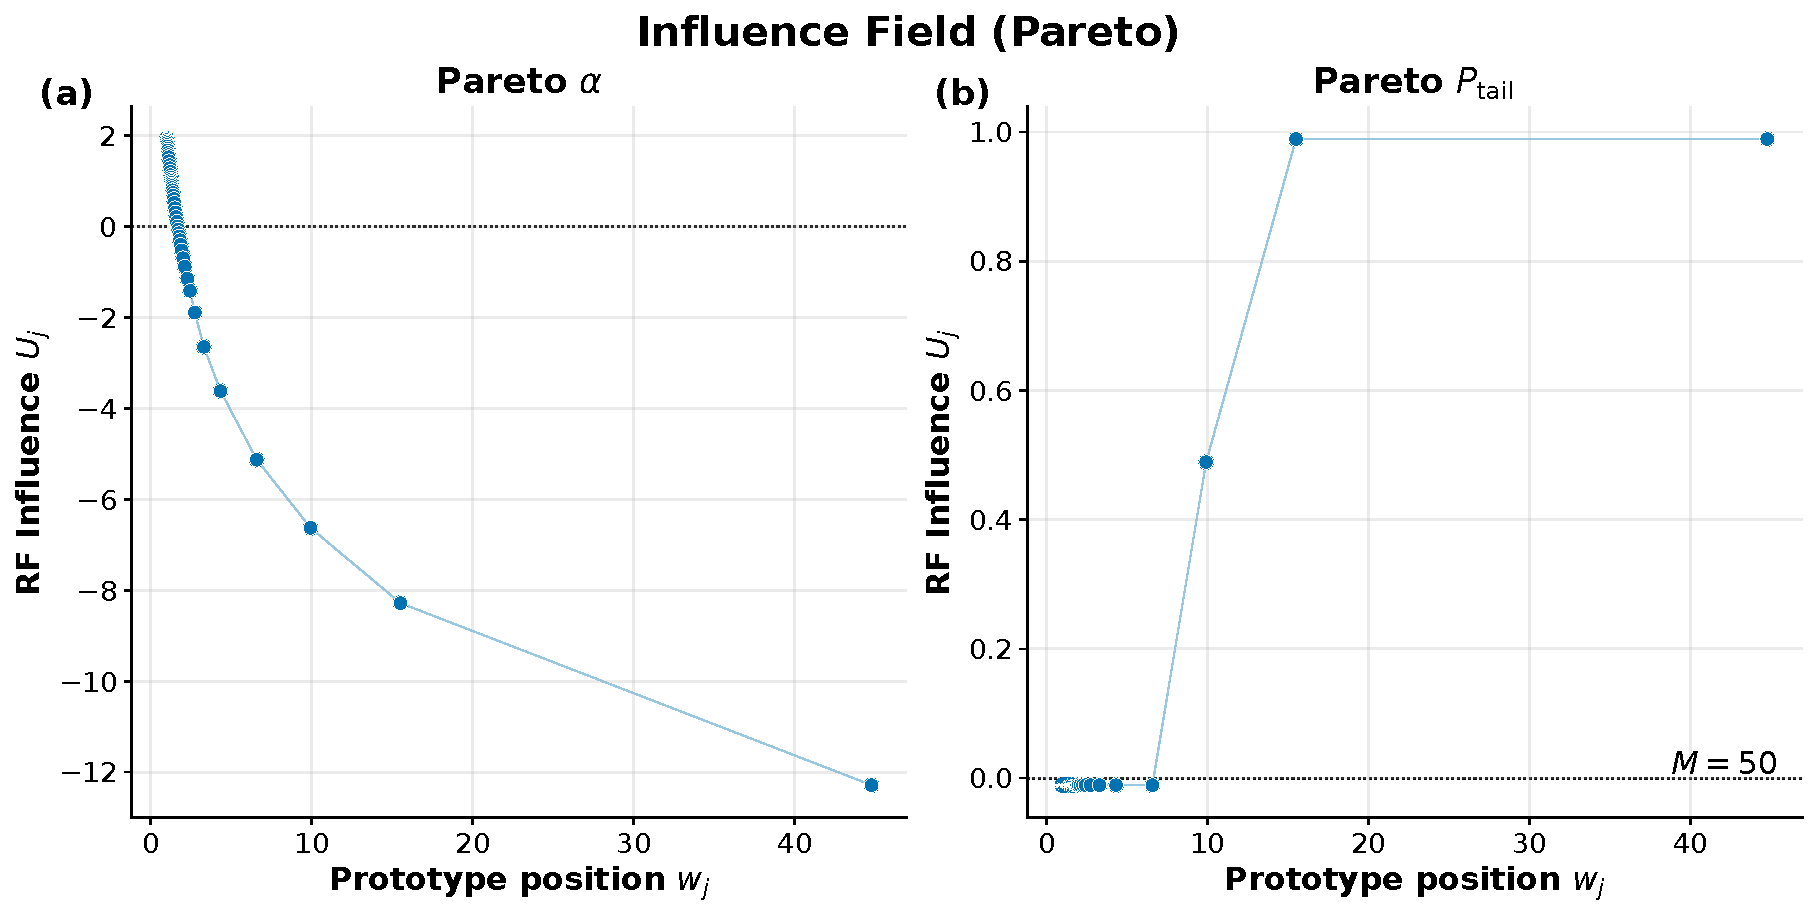
\includegraphics[width=\linewidth]{f9.pdf}
\caption{
RF influences~\eqref{eq:Uj} for two Pareto estimands on a
single fitted partition ($N = 1000$, $M = 50$). In one dimension each
prototype $w_j$ is a scalar, so the horizontal axis orders the receptive
fields in data space. (a) For the shape parameter $\alpha$, $U_j$
varies across the partition, so the RF influence averages are informative and the between-RF term carries the variance. (b) For the tail probability
$P(X > c)$ with $c$ the $0.99$ quantile, $\psi$ takes rouhgly values and
$U_j$ is constant within every RF that does not straddle $c$. 
}
\label{fig:field}
\end{figure}

% ======================================================================
\section{Experimental Data}\label{sec:data}
% ======================================================================

We evaluate QIJ on three datasets. Two are from distributional families in which the ground truth is known, and one is a real-world model from observational astronomy with vector-valued estimands. In what follows, $S=1000$ Monte Carlo draws of size $N = 1000$ were taken from each data process. QIJ and a standard nonparametric bootstrap ($B = 2000$ replicates) were run on identical draws paired by seed. For QIJ, we quantize with $k$-means, where the number of prototypes $M$ varies along a grid.  The astronomical case uses an empirical population protocol where a large catalog is treated as the population, draws are sampled from it with replacement, and the target $\theta_{\mathrm{true}}$ is taken to be the parameter vector computed from the full catalog. Below, we describe the datasets individually.

\paragraph{Pareto.} A heavy-tailed distribution, with closed-form influence functions for both estimators (the shape parameter's maximum-likelihood estimator, and a tail probability), so every stage of the pipeline can be checked analytically ($M$ grid from 20 to 128).

\paragraph{Multivariate $t$ (MVT).} A ten-dimensional, elliptically symmetric distribution with two estimands: the degrees of freedom $\nu$ (estimated by profile maximum likelihood), and a tail probability. This tests whether our  construction survives higher data dimension ($M$ grid from 10 to 100).

\paragraph{Galaxy fundamental plane.} The galaxy Fundamental Plane dataset (FP) comprises 76{,}997 early-type galaxies drawn from the Sloan Digital Sky Survey Data Release 7 spectroscopic catalog \cite{abazajian2009}. 
%Galaxies were selected in the redshift range $0.05 \le z \le 0.10$ with reliable velocity dispersion measurements ($\sigma > 70~\mathrm{km\,s^{-1}}$, $\sigma_{\mathrm{err}} < 30~\mathrm{km\,s^{-1}}$) and concentration indices $r_{90}/r_{50} > 2.5$ to isolate early-type morphologies. 
For each galaxy, the three Fundamental Plane observables are the aperture-corrected stellar velocity dispersion $\sigma$ (following the correction of \cite{jorgensen1995}), the 
%de Vaucouleurs 
effective radius $R_e$ 
%converted to physical kpc using a standard $\Lambda$CDM cosmology ($H_0 = 70~\mathrm{km\,s^{-1}\,Mpc^{-1}}$, $\Omega_m = 0.3$)
, and a luminosity-based surface brightness proxy $I_e$.
%$I_e = L_r/(2\pi R_e^2)$ derived from the extinction-corrected $r$-band apparent magnitude. 
The Fundamental Plane is fit in log-space as $\log R_e = a\,\log\sigma + b\,\log I_e + c$ via least squares. The estimands are the coefficient vector $(a,b,c)$ and the intrinsic scatter about the plane ($M$ grid from 8 to 128).


% ======================================================================
\section{Results}\label{sec:results}
% ======================================================================

\subsection{Examining the Variance Decomposition}\label{sec:res-valid}

Because the left side of \eqref{eq:identity} contains no $M$-dependence, it is  constant with respect to the number of prototypes used to quantize the data. Figure~\ref{fig:invariance} confirms this, with each component of \eqref{eq:identity} averaged across the $S = 1000$ Monte Carlo draws: $\Vcell$ rises ($\Vwithin$ falls) as the partition refines, but their sum is flat. %Panel (a) also quantifies the split: for the one-dimensional Pareto, $\Vcell$ is more than two orders of magnitude higher than $\Vwithin$, meaning the perturbation responses $U_j$ carry almost all of the variance information in this case.

\begin{figure}[t]
\centering
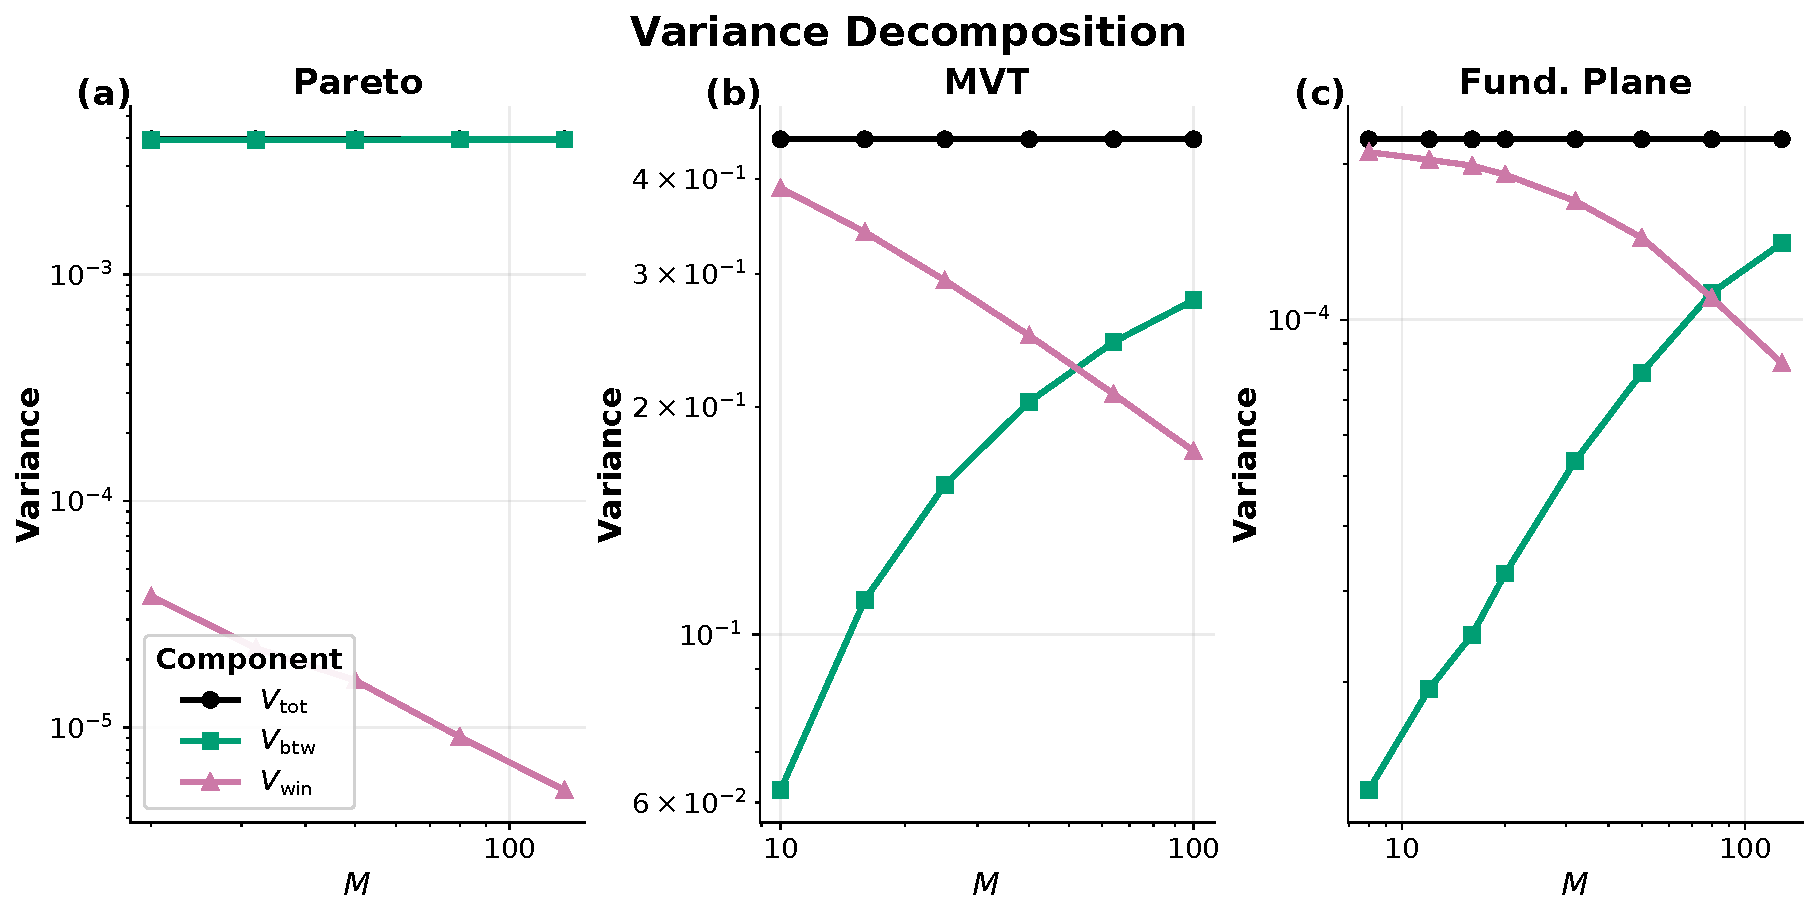
\includegraphics[width=\linewidth]{f3.pdf}
\caption{
%The variance decomposition (eq.~\eqref{eq:identity}) is partition-invariant. 
Each panel shows the three terms of ~\eqref{eq:identity}) against increasing $M$ (finer quantization), averaged over the $S = 1000$ Monte Carlo draws. As the partition refines, the between-RF term $V_\mathrm{btw}$ (squares)
rises and the within-RF term $V_\mathrm{win}$ (triangles) falls, while
their sum $V_\mathrm{tot}$ (circles) is constant in $M$. (a) show the decomposition for the Pareto shape parameter; (b) shows the MVT degrees of freedom $\nu$; (c) shows the FP coefficient $a$. 
}
\label{fig:invariance}
\end{figure}



\subsection{Validation against the Bootstrap}

The estimator variances shown in Figure~\ref{fig:invariance} are similar to those identified by the standard bootstrap, which is reported in Figure~\ref{fig:coverage}(a), broken out by estimand. The paired ratio $\log(V_{\mathrm{QIJ}}/V_{\mathrm{boot}})$ conveys agreement ($=0$) or disagreement ($\neq 0$) of QIJ's estimated sampling variance, compared to that of the standard bootstrap. Offsets of order $1/N$ are expected, since QIJ omits higher-order terms and the bootstrap carries its own $O(1/N)$ bias.
Figure~\ref{fig:coverage}(b) compares nominal and empirical coverage of the two interval estimators; QIJ tracks the unity slope, whereas standard bootstrap is mildly conservative at low nominal levels; at commonly used levels (0.90 and above) both methods are nominal within Monte Carlo error (gray shaded band). Figure~\ref{fig:coverage}(c) compares mean interval widths from both methods at the nominal level at which each method attains 95\% empirical coverage (0.955 for QIJ, 0.949 for the bootstrap): the width ratios lie between 1.004 and 1.065, largest for the two tail-probability estimands.

\begin{figure}[t]
\centering
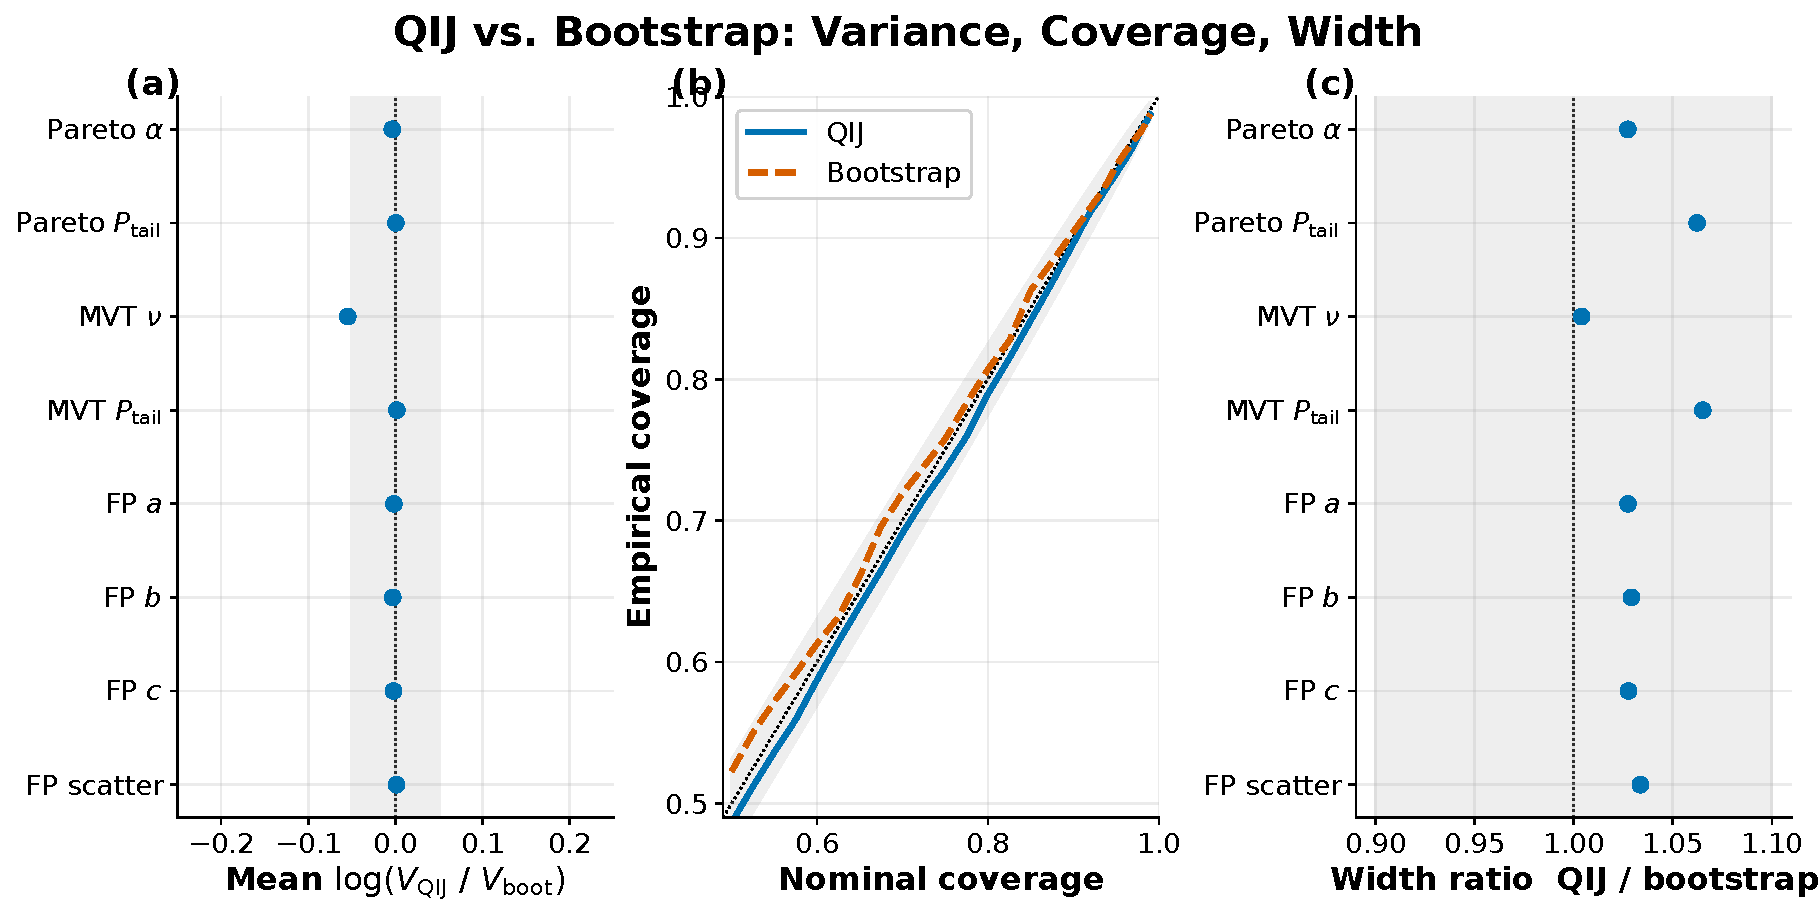
\includegraphics[width=\linewidth]{f2.pdf}
\caption{Validation against the standard bootstrap. (a) Mean $\log(V_{\mathrm{QIJ}}/V_{\mathrm{boot}})$ per estimand, with 95\% CI whiskers (smaller than the markers at $S = 1000$); the shaded band marks $\pm 0.05$. All estimands fall inside the band except the MVT $\nu$, just outside at $-0.055$. (b) Empirical versus nominal coverage, pooled over all datasets and estimands, overlaid on the $\pm 1.96\sqrt{p(1-p)/S}$ Monte Carlo standard error band. QIJ tracks the diagonal cleanly, whereas the bootstrap is mildly conservative at low nominal levels. 
%and both are nominal at common levels (e.g., 0.90, 0.95, 0.99). 
(c) Mean interval width ratios (QIJ over bootstrap)  evaluated at the nominal level where each method attains 0.95 level empirical coverage (0.955 for QIJ, 0.949 for the bootstrap); the shaded band marks $\pm 10\%$. The ratios range from 1.004 to 1.065, with the largest for the tail-probability estimands.}
\label{fig:coverage}
\end{figure}

\subsection{The Computation-Accuracy Frontier}\label{sec:res-compute}

To produce the intervals presented in Figure~\ref{fig:coverage}, QIJ demands a number of evaluations of $T$ that scales with $M$ rather than with $B$. Compared to the standard bootstrap, where hundreds to thousands of replicates (and associated $T$ evaluations) are needed, this is one to two orders of magnitude cheaper. To demonstrate this cost savings, Figure~\ref{fig:compute} shows the interval width each method achieves as a function of the number of evaluations of $T$ when estimating the $\sigma$ (velocity dispersion) slope of the galaxy Fundamental Plane data. The intervals in Figure~\ref{fig:compute} are computed from analytic influence functions and plotted at the location $M{+}1 = 51$ that QIJ occupies when numerical derivaties are required to estimate its influence funtions $\psi$. The standard bootstrap does not match this width until $b \approx 1800$ replicates/$T$ evaluations have occurred (the figure shows all widths relative to that computed from the standard bootstrap's width after 2000 replicates). Both methods target the same population coefficient $a$, but QIJ achieves widths comparable to the standard bootstrap with far fewer ($51 \ll {\sim}1800$) estimator evaluations.

\begin{figure}[t]
\centering
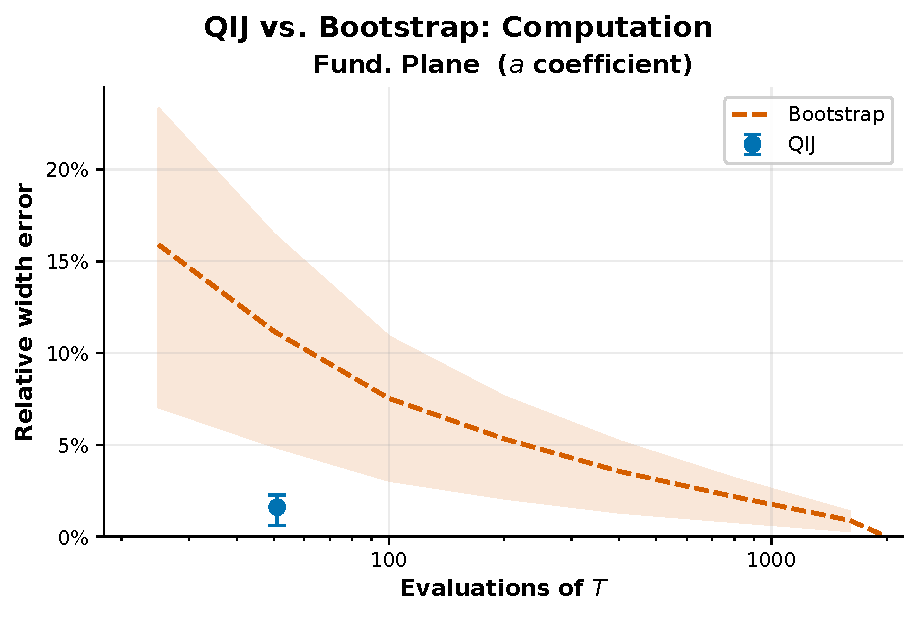
\includegraphics[width=.85\linewidth]{f7.pdf}
\caption{Computation frontier on the FP coefficient $a$. For each Monte Carlo draw, the bootstrap 95\% interval width is recomputed from the first $b$ replicates (in sequence) and then compared to the full $B = 2000$ reference (dashed line: mean over the $S = 1000$ draws; ribbon: interquartile range); the error at $b = B$ is zero by construction. The QIJ point shows the width of QIJ's deterministic interval against the same converged bootstrap reference (interquartile range as whiskers). The width is computed from analytic influence functions and plotted at the abscissa $M{+}1 = 51$ that QIJ's derivative-free route would require when $M = 50$. QIJ's width is partition-invariant (see Fig.~\ref{fig:invariance}), so a single operating point suffices. The standard bootstrap does not achieve the width accuracy of QIJ intervals until replicate $\sim$1800 (cumulatively requiring $\sim$1800 estimator evaluations).}
\label{fig:compute}
\end{figure}

% ======================================================================
\section{Conclusions and Future Work}\label{sec:conclusions}
% ======================================================================

%We have shown that a fitted vector quantizer supports nonparametric interval estimation. The route is not resampling from the partition; this would require variability that the quantizer itself minimizes away. Instead, we harness the Voronoi partition learned by the VQ to study perturbations of estimator influence across the learned manifold. In a VQ setting, bootstrap resampling can be re-cast as a process of changing RF counts. By analyzing an estimator's sensitivity to these changing counts \textit{locally} (across the learned manifold), we can construct a notion of global estimator variance, which we use to power QIJ's interval estimation. Across our three test cases, including a real astronomical problem with empirically derived truth, QIJ delivers nominal coverage at bootstrap-matched widths, at a small fraction of the computation.

We have shown that a fitted vector quantizer supports nonparametric
interval estimation. The route to this is not via resampling from the partition, which would require the same sampling variability that the quantizer minimizes away, but, instead, differentiation across it. The receptive fields supply a coarse basis in which bootstrap resampling becomes a redistribution of counts whose multinomial fluctuations are known, and the estimator's sensitivity to those counts is measurable in a number of evaluations set by $M$, rather than $B$. This construction relies on the variance decomposition of \eqref{eq:identity}, which is an algebraic identity on any dataset and any partition. 

Across eight estimands on three datasets, including a real astronomical problem with empirically derived truth, QIJ's variance estimates agree with
the bootstrap's to within $0.05$ (in log-ratio) for all but one; its
intervals track nominal coverage across the level grid; and its widths fall
within $7\%$ of bootstrap widths. QIJ inherits the infinitesimal jackknife's requirement that the estimator be smooth in the data weights, and it estimates variance without correcting bias.

This work is an attempt at harnessing VQ in the specification and study of uncertainty quantification. Our study has revealed several directions for future work, including how VQs should be prescribed (i.e., how many prototypes used for quantization) when the goal is inference rather than compression, which could be useful for inference in large full catalogs of data.

\begin{credits}
\subsubsection{\ackname} JT and SSRO acknowledge support from NSF AAG 2107942, NASA ADAP 80NSSC23K0476, and the US NSF under Cooperative Agreement 2421782 and the Simons Foundation grant MPS-AI-00010515 awarded to the NSF-Simons AI Institute for Cosmic Origins --- CosmicAI, \url{https://www.cosmicai.org/}. SSRO also acknowledges support from a Peter O'Donnell Distinguished Researcher Fellowship and a Donald Harrington Fellowship.
\subsubsection{\discintname} The authors have no competing interests to declare.
\end{credits}

\bibliographystyle{splncs04}
\bibliography{refs}

\end{document}
